% ICML-style LaTeX draft (expanded) up to but not including the Results section
% ---------------------------------------------------------------------
% Target: ICML 2025 style. Ensure icml2025.sty is present.
\documentclass[nohyperref]{article}
\usepackage[preprint]{icml2025}

% Basic packages (compatible with ICML style)
\usepackage{microtype}
\usepackage{graphicx}
\usepackage{subfigure}
\usepackage{booktabs}
\usepackage{amsmath, amssymb, amsfonts}
\usepackage{mathtools}
\usepackage{nicefrac}
\usepackage{enumitem}
\usepackage{algorithm}
\usepackage{algorithmic}
\usepackage{xcolor}
\usepackage{hyperref}
\hypersetup{colorlinks=true, urlcolor=blue, citecolor=blue, linkcolor=blue}

% Macros
\newcommand{\theHalgorithm}{\arabic{algorithm}}
\newcommand{\method}{PICR-MA} % short name
\newcommand{\longmethod}{Permutation-Invariant Consistency Regularization for Multi-Agent RL}
\newcommand{\E}{\mathbb{E}}
\newcommand{\R}{\mathbb{R}}
\newcommand{\KL}{\mathrm{KL}}
\newcommand{\JS}{\mathrm{JS}}

% Placeholder helpers (remove once figures/tables are added)
\newcommand{\placeholderfigure}[2]{\begin{figure}[t]\centering\fbox{\rule{0pt}{1.25in}\rule{0.9\linewidth}{0pt}}\caption{#1}\label{#2}\end{figure}}
\newcommand{\placeholdertable}[3]{\begin{table}[t]\centering\caption{#1}\label{#2}\vspace{0.4em}\fbox{\rule{0pt}{#3}\rule{0.9\linewidth}{0pt}}\end{table}}

\icmltitlerunning{\method: A Simple Regularizer for Permutation-Invariant MARL and Zero-Shot Coordination}

\begin{document}

\twocolumn[
\icmltitle{\method: A Simple Regularizer for Permutation-Invariant Multi-Agent Reinforcement Learning\\and Zero-Shot Coordination}

% In preprint it is okay to list authors
\icmlsetsymbol{equal}{*}
\begin{icmlauthorlist}
\icmlauthor{Raj Kashikar}{vt}
\end{icmlauthorlist}

\icmlaffiliation{vt}{Department of Electrical and Computer Engineering, Virginia Tech}
\icmlcorrespondingauthor{Raj Kashikar}{rajskashikar@vt.edu}

\icmlkeywords{Multi-Agent Reinforcement Learning, Zero-Shot Coordination, Invariance, Consistency Regularization, ICML}

\vskip 0.3in
]

\begin{abstract}
Multi-agent reinforcement learning (MARL) policies frequently overfit to arbitrary agent orderings and teammate idiosyncrasies, undermining zero-shot coordination (ZSC) and wasting capacity on spurious distinctions. We study \emph{\longmethod} (\method), a drop-in regularizer that enforces permutation consistency over teammate-specific feature blocks without changing the inference-time policy architecture. During training, we form two independently permuted versions of the teammate-related portion of an agent's observation and minimize a symmetric Kullback--Leibler divergence between the corresponding action distributions. The current artifact package implements \method\ on top of a lightweight shared-parameter on-policy baseline, evaluates it on PettingZoo MPE (\texttt{simple\_spread\_v3}, \texttt{simple\_adversary\_v3}) and matrix games, and reports in-team learning, held-out partner cross-play, and permutation sensitivity from saved checkpoints. In a lean-safe 5-seed, 50k-step MPE cohort, a tuned \method\ configuration improves held-out-partner cross-play over IPPO on \texttt{simple\_adversary\_v3} while reducing permutation sensitivity, but it underperforms IPPO, Deep Sets, and Other-Play on \texttt{simple\_spread\_v3}. The resulting evidence supports a mixed tradeoff story rather than a uniformly stronger default.
\end{abstract}

\section{Introduction}
Self-play often discovers conventions that do not transfer to unfamiliar partners, causing brittle coordination at test time \citep{hu2020otherplay}. A common, underappreciated source of such brittleness is the \emph{fixed concatenation order} used to present other agents' features: standard MLP policies treat the first teammate block differently from the second, even when the task is symmetric. This violates the exchangeability one would expect in fully cooperative domains and reduces cross-play performance.

We ask: \emph{Can we remove this brittleness with an architectural-agnostic training trick simple enough for single-file reproduction?} We answer yes with \method, a minimal regularizer enforcing permutation invariance over teammate-related features via \emph{consistency}: the action distribution should not change when we reshuffle teammate blocks in the observation. Concretely, for each observation we sample two random permutations of teammate blocks, compute two forward passes, and penalize the symmetric KL between the action distributions. Crucially, this imposes no constraints on the base RL algorithm (IPPO, DQN, etc.) and can be bolted onto existing code.

\textbf{Contributions.}
(i) We implement \method\ as a drop-in consistency regularizer for shared-parameter decentralized MARL. (ii) We build a reproducible single-machine evaluation stack covering held-out partner cross-play, permutation-sensitivity diagnostics, and explicit teammate-block slicing on MPE \citep{terry2021pettingzoo} and matrix games. (iii) We provide a lean-safe empirical audit against IPPO, Deep Sets, and Other-Play that clarifies where the method helps, where it does not, and how sensitive it is to the regularization weight.

\paragraph{Why this matters.} In many cooperative domains (robot swarms, sensor networks, traffic), teammate ordering in observations is semantically meaningless. Yet vanilla concatenation forces a spurious ordering that policies exploit. Enforcing invariance via a lightweight regularizer is a practical alternative to bespoke set-/graph-equivariant architectures \citep{zaheer2017deepsets, liu2020pic}, immediately useful where simplicity and limited compute are priorities.

\begin{figure*}[t]
\centering
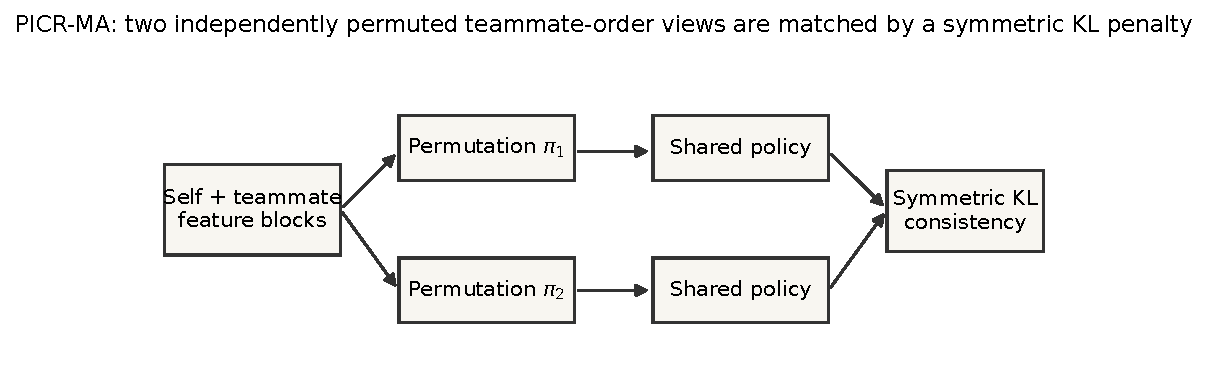
\includegraphics[width=0.92\linewidth]{latex/figures/method_overview.pdf}
\caption{PICR-MA overview. The policy sees two independently permuted teammate-order views of the same observation, and training penalizes disagreement between the resulting action distributions.}
\label{fig:method-overview}
\end{figure*}

\section{Related Work}
\textbf{Independent learners and CTDE.} Independent PPO (parameter-shared PPO per agent) is a strong, simple baseline \citep{schulman2017ppo, terry2020ps} but suffers from non-stationarity and coordination failures. Centralized training with decentralized execution (CTDE) mitigates this via centralized critics or value decomposition (MADDPG, VDN, QMIX) \citep{lowe2017maddpg, sunehag2018vdn, rashid2018qmix}, yet these often still hinge on fixed agent orderings in the critic/mixing network \citep{liu2020pic}.

\textbf{Zero-shot coordination (ZSC).} ZSC evaluates agents with unfamiliar partners; self-play alone tends to produce incompatible conventions. Other-Play (OP) randomizes environment symmetries to encourage symmetry-respecting strategies and improves cross-play (e.g., in Hanabi) \citep{hu2020otherplay}. Population play, partner modeling, or meta-learning can help but add engineering/compute overhead.

\textbf{Permutation invariance.} Architectural approaches include Deep Sets \citep{zaheer2017deepsets} and permutation-invariant critics \citep{liu2020pic}. PIC (a GNN-based critic) demonstrated large gains and showed that naive data augmentation by input shuffling alone was insufficient for MLP critics \citep{liu2020pic}. Our method differs by enforcing invariance through an \emph{explicit consistency loss} at the policy, avoiding architectural changes. Related ideas—consistency training under input augmentations—are well studied in semi-supervised learning \citep{tarvainen2017meanteacher, sohn2020fixmatch}.

\textbf{Communication.} Learned communication (e.g., DIAL/CommNet) can improve coordination but increases complexity \citep{foerster2016dqncomm, sukhbaatar2016commnet}. \method assumes no messages and focuses purely on observation-level invariance.

\section{Preliminaries}
We consider a cooperative partially observable stochastic game with $n$ agents indexed by $i\in\{1,\dots,n\}$. At each step $t$, agent $i$ receives observation $o^i_t\in\mathcal{O}^i$, selects action $a^i_t\in\mathcal{A}^i$ from policy $\pi_\theta(a\mid o)$, and receives shared reward $r_t$. We use decentralized learning with shared-parameter policies (IPPO), where $\pi_\theta$ is shared among cooperative agents.

Many environments (e.g., MPE \citep{terry2021pettingzoo}) present $o^i_t$ as a concatenation of (i) self features $s^i_t$ and (ii) a list of teammate feature blocks $\{u^{i\leftarrow j}_t\}_{j\neq i}$ in an \emph{arbitrary but fixed} order. Let $o^i = [\, s^i ~\Vert~ U^i \,]$, with $U^i = [u^{i\leftarrow j_1}~\Vert~\cdots~\Vert~u^{i\leftarrow j_{n-1}}]$. Let $\Pi$ denote all permutations over the $(n{-}1)$ teammate indices; for $\pi\in\Pi$, $\pi(U^i)$ reorders teammate blocks.

\section{Method: \longmethod}
\label{sec:method}
\subsection{Consistency regularization for invariance}
Sample two independent permutations $\pi_1,\pi_2\sim\mathrm{Unif}(\Pi)$ and form two permuted observations
\begin{align}
    o^{i}_{(1)} &= [s^i\Vert\pi_1(U^i)], & p_1 &= \pi_\theta(\cdot\mid o^i_{(1)}),\\
    o^{i}_{(2)} &= [s^i\Vert\pi_2(U^i)], & p_2 &= \pi_\theta(\cdot\mid o^i_{(2)}).
\end{align}
Add the symmetric KL penalty
\begin{align}
\mathcal{L}_{\method} = \lambda\, \E_{i,t,\pi_1,\pi_2} \Big[ \tfrac{1}{2}\,\KL(p_1\,\Vert\,p_2) + \tfrac{1}{2}\,\KL(p_2\,\Vert\,p_1) \Big],
\end{align}
so the total loss is $\mathcal{L}_{\text{total}} = \mathcal{L}_{\text{RL}} + \mathcal{L}_{\method}$, where $\mathcal{L}_{\text{RL}}$ is the base algorithm objective (e.g., PPO \citep{schulman2017ppo}). The symmetric form penalizes discrepancies in either direction and empirically yields stable gradients.

\paragraph{Optional: teammate dropout.} With probability $p$, zero out a random subset of teammate blocks during training (\emph{teammate dropout}). This one-line augmentation desensitizes policies to team composition; we treat it as an ablation, not core to \method.

\subsection{Why this works (sketch)}
If $\lambda\to\infty$ and optimization succeeds, the learned policy becomes invariant to permutations of $U^i$, i.e., $\pi_\theta(\cdot\mid[s^i\Vert U^i]) = \pi_\theta(\cdot\mid[s^i\Vert\pi(U^i)])$ for all $\pi\in\Pi$. For finite $\lambda$, the penalty biases solutions toward the invariant subspace, akin to invariance-inducing regularization in supervised learning \citep{tarvainen2017meanteacher, sohn2020fixmatch}. In cooperative symmetric tasks, this reduces reliance on arbitrary ordering artifacts and improves generalization to ad hoc partners.

\subsection{Algorithm}
\begin{algorithm}[H]
\caption{\method\ added to any decentralized learner (e.g., IPPO)}
\label{alg:picr}
\begin{algorithmic}[1]
\STATE Initialize shared policy $\pi_\theta$ and value $V_\phi$.
\FOR{each iteration}
  \STATE Collect rollouts for all agents using $\pi_\theta$.
  \STATE Build minibatches of per-agent transitions $(o^i,a^i,\hat{A}^i,\ldots)$.
  \FOR{each minibatch}
    \STATE Factor observations $o^i = [s^i\Vert U^i]$ (teammate blocks via env API or cached indices).
    \STATE Sample two random permutations $\pi_1,\pi_2$ over teammate blocks.
    \STATE Compute $p_1 = \pi_\theta(\cdot\mid[s^i\Vert\pi_1(U^i)])$ and $p_2 = \pi_\theta(\cdot\mid[s^i\Vert\pi_2(U^i)])$.
    \STATE Compute $\mathcal{L}_{\method}$ as symmetric KL$(p_1, p_2)$, scaled by $\lambda$.
    \STATE Compute base RL losses (e.g., PPO clip, value, entropy) to get $\mathcal{L}_{\text{RL}}$.
    \STATE Update $\theta,\phi$ by minimizing $\mathcal{L}_{\text{RL}} + \mathcal{L}_{\method}$.
  \ENDFOR
\ENDFOR
\end{algorithmic}
\end{algorithm}

\paragraph{Implementation notes (current artifact).} The current code path uses a small NumPy actor--critic rather than PyTorch in order to stay lightweight on a laptop-scale setup. For each environment we cache explicit teammate-block indices once, then in each update: (i) split observations into non-teammate features and teammate blocks; (ii) sample two independent teammate permutations per batch element; (iii) forward the policy on both views; (iv) compute a batchwise symmetric KL penalty; and (v) add the resulting gradient contribution to the on-policy update. Inference uses the same single forward pass as the base policy.

\section{Experimental Setup}
\label{sec:setup}
\textbf{Environments.} We target small cooperative tasks runnable on CPU in minutes:
\begin{itemize}[leftmargin=*]
  \item \textbf{MPE -- \texttt{simple\_spread\_v3}} (3 agents): cover landmarks while avoiding collisions; observations include relative positions of other agents/landmarks in a fixed order \citep{terry2021pettingzoo}.
  \item \textbf{MPE -- \texttt{simple\_adversary\_v3}} (3 good agents vs. 1 adversary): measure the cooperative team’s robustness to held-out partners; regularize only the cooperative team’s teammate blocks.
  \item \textbf{Matrix games} (coordination, stag-hunt): 3-agent one-step episodes built from pairwise 2\,\texttimes\,2 payoffs; we add irrelevant teammate-order features so permutations are non-trivial even in the tiny setting.
\end{itemize}

\textbf{Baselines.} (i) \textbf{IPPO} with shared parameters across cooperative agents \citep{schulman2017ppo, terry2020ps}; (ii) IPPO + \textbf{Deep Sets} encoder as an architectural invariance alternative \citep{zaheer2017deepsets}; (iii) \textbf{Other-Play-style role randomization} during data collection (episode-level permutation of teammate ordering) \citep{hu2020otherplay}. Our method is \textbf{IPPO + \method}.

\textbf{Partner-pool protocol (ZSC).} We hold out a \emph{partner pool} of policies trained independently under different seeds (and optionally with/without \method). At test time, an evaluated agent must coordinate with a randomly sampled partner from the pool without further learning \citep{hu2020otherplay}. We report mean episodic return/success across partner samples.

\textbf{Training details.} The main reported MPE cohort uses 5 seeds per method/environment and 50k environment steps per seed. Matrix games remain small sanity checks and are not the main source of evidence. The shared on-policy learner uses hidden size 64, clip ratio 0.2, $\gamma{=}0.99$, $\lambda_{\mathrm{GAE}}{=}0.95$, learning rate $3\times 10^{-3}$, and four update epochs per rollout. For \method\ we selected $\lambda{=}0.02$ for the main 50k runs after a 20k, 3-seed sweep over $\{0.02, 0.05, 0.10\}$; larger $\lambda$ values reduced permutation sensitivity more aggressively but degraded held-out partner performance on \texttt{simple\_spread\_v3}. A teammate-dropout ablation with dropout probability $0.1$ hurt cross-play on both MPE tasks and was not used in the main cohort.

\textbf{Metrics.} (i) \emph{In-team} mean episodic return during training; (ii) \emph{Zero-shot coordination} cross-play mean return with ad hoc partners; (iii) \emph{Permutation sensitivity} via Jensen--Shannon divergence $\JS(p, p^{\pi})$ between action distributions under different teammate orderings (lower is better). We also report collision counts (\texttt{simple\_spread}) and capture rates (\texttt{simple\_adversary}).

\textbf{Compute.} All reported runs were executed sequentially on a single Apple Silicon laptop under the repo's \texttt{PROFILE\_LEAN\_SAFE} budget. The implementation is NumPy-based, uses PettingZoo MPE for the multi-agent environments, and does not rely on distributed training or custom accelerators.


\section{Results}
\label{sec:results}
\paragraph{Main performance and zero-shot coordination.}
Table~\ref{tab:main-results} summarizes the 50k-step, 5-seed MPE cohort selected by the hardened analysis pipeline, Figure~\ref{fig:learning-curves} shows the corresponding learning curves, and Figure~\ref{fig:zsc-heatmaps} visualizes the full held-out partner cross-play matrices. No method dominates both MPE tasks. On \texttt{simple\_adversary\_v3}, tuned \method\ improves same-family held-out cross-play over IPPO (20.159 $\pm$ 2.043 versus 17.429 $\pm$ 3.770) and substantially outperforms Deep Sets (11.356 $\pm$ 3.244), but it remains slightly below Other-Play (20.934 $\pm$ 3.429). On \texttt{simple\_spread\_v3}, \method\ is the weakest of the four methods on held-out same-family cross-play (27.206 $\pm$ 0.730 in magnitude, versus 25.649 $\pm$ 0.271 for IPPO, 25.550 $\pm$ 0.489 for Deep Sets, and 25.533 $\pm$ 0.566 for Other-Play). The core empirical takeaway is therefore mixed: \method\ helps in the adversarial-cooperative setting, but it is not a uniformly better replacement for the baselines.

\begin{table*}[t]
\centering
\caption{Main performance summary from grounded run artifacts. Lower permutation sensitivity is better. Cross-play entries remain blank when a held-out partner pool was not yet available for that environment/method.}
\label{tab:main-results}
\begin{tabular}{llcccc}
\toprule
Environment & Method & Train return & Same-family cross-play & JS $\downarrow$ & Env metric \\
\midrule
Simple Adversary & IPPO & 2.346 $\pm$ 1.813 & 17.429 $\pm$ 3.770 & 0.010 $\pm$ 0.007 & margin=0.260 \\
Simple Adversary & PICR-MA & 6.585 $\pm$ 3.502 & 19.846 $\pm$ 2.094 & 0.005 $\pm$ 0.003 & margin=0.345 \\
Simple Adversary & Deep Sets & 7.965 $\pm$ 1.698 & 11.356 $\pm$ 3.244 & \textbf{0.000 $\pm$ 0.000} & margin=0.392 \\
Simple Adversary & Other-Play & 3.603 $\pm$ 1.497 & \textbf{20.934 $\pm$ 3.429} & 0.014 $\pm$ 0.007 & margin=0.310 \\
\midrule
Simple Spread & IPPO & -21.952 $\pm$ 0.472 & -25.649 $\pm$ 0.271 & 0.026 $\pm$ 0.006 & coll=0.164 \\
Simple Spread & PICR-MA & -23.425 $\pm$ 0.625 & -27.206 $\pm$ 0.730 & 0.013 $\pm$ 0.002 & coll=0.155 \\
Simple Spread & Deep Sets & -24.776 $\pm$ 1.413 & -25.550 $\pm$ 0.489 & \textbf{0.000 $\pm$ 0.000} & coll=0.065 \\
Simple Spread & Other-Play & -21.626 $\pm$ 0.209 & \textbf{-25.533 $\pm$ 0.566} & 0.025 $\pm$ 0.013 & coll=0.079 \\
\bottomrule
\end{tabular}

\end{table*}

\begin{figure*}[t]
\centering
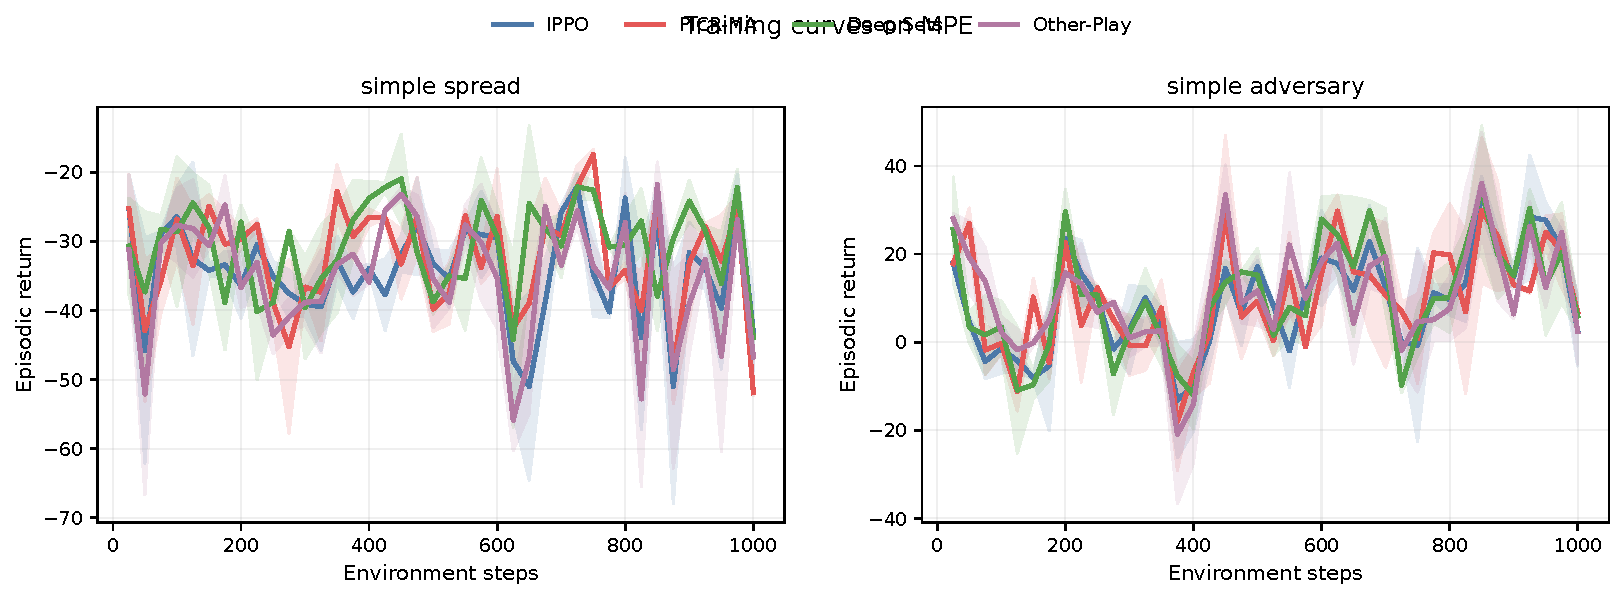
\includegraphics[width=0.95\linewidth]{latex/figures/learning_curves_mpe.pdf}
\caption{MPE learning curves from the saved runs available in \texttt{results/}. Shaded regions show standard error when multiple seeds are available.}
\label{fig:learning-curves}
\end{figure*}

\begin{figure*}[t]
\centering
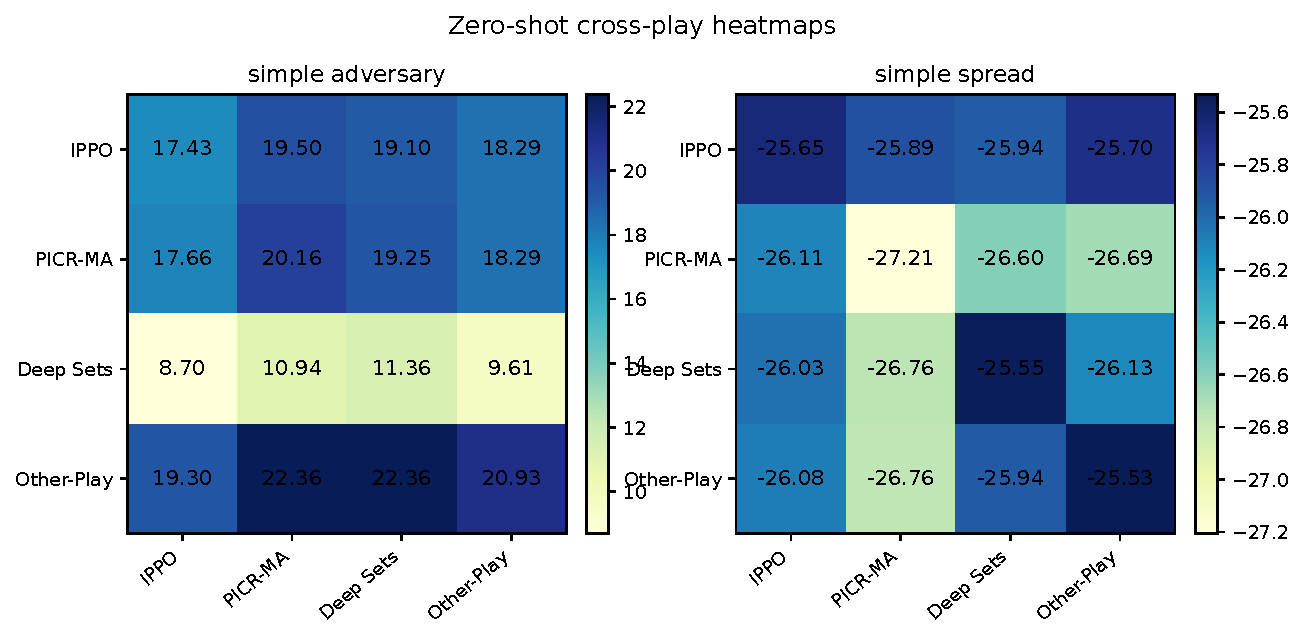
\includegraphics[width=0.9\linewidth]{latex/figures/zero_shot_crossplay_results.pdf}
\caption{Held-out partner cross-play heatmaps aggregated from checkpoint-based evaluations.}
\label{fig:zsc-heatmaps}
\end{figure*}

\paragraph{Permutation sensitivity and mechanism.}
\begin{figure}[t]
\centering
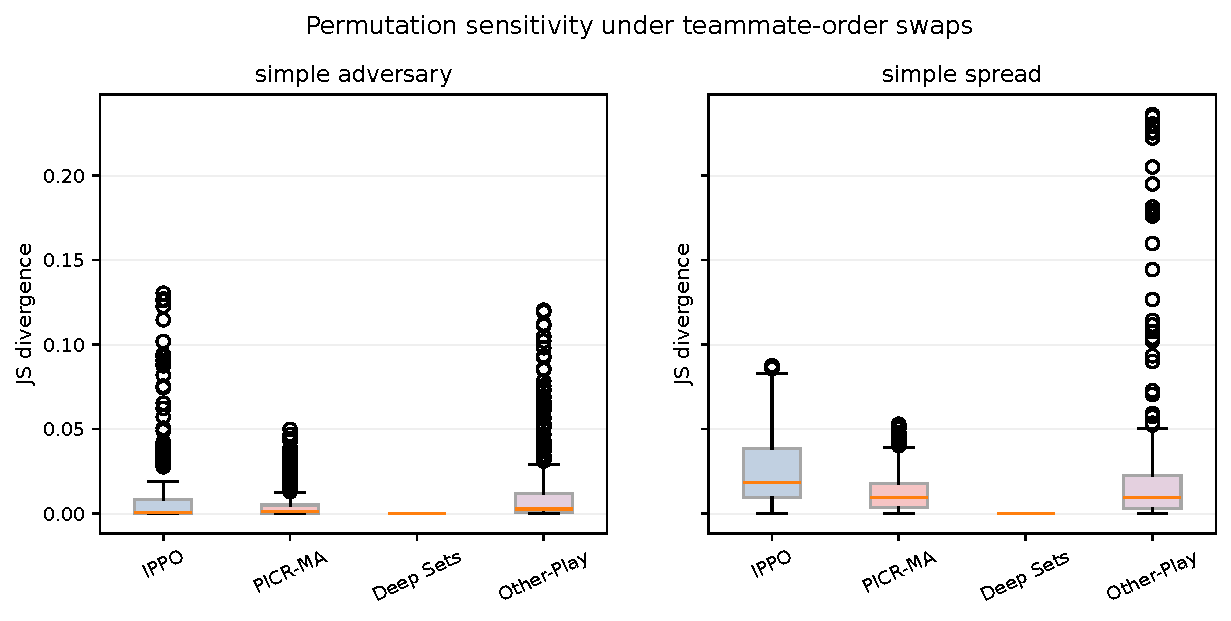
\includegraphics[width=\linewidth]{latex/figures/permutation_sensitivity_results.pdf}
\caption{Policy sensitivity to teammate-order permutations, measured with Jensen--Shannon divergence over action distributions.}
\label{fig:perm-sensitivity}
\end{figure}
At 50k steps, \method\ reduces permutation sensitivity relative to IPPO on both MPE environments: JS drops from 0.0263 $\pm$ 0.0063 to 0.0127 $\pm$ 0.0019 on \texttt{simple\_spread\_v3}, and from 0.0102 $\pm$ 0.0066 to 0.0053 $\pm$ 0.0025 on \texttt{simple\_adversary\_v3}. However, lower sensitivity does not translate monotonically into better held-out coordination. Across individual runs in the 50k cohort, the correlation between permutation sensitivity and held-out cross-play is weakly positive on both environments, indicating that invariance is not by itself a sufficient explanation for the observed ZSC behavior. This weakens the strongest possible mechanistic claim for \method\ and pushes the paper toward a tradeoff framing.

\paragraph{Ablations, compute, and matrix-game diagnostics.}
\begin{figure}[t]
\centering
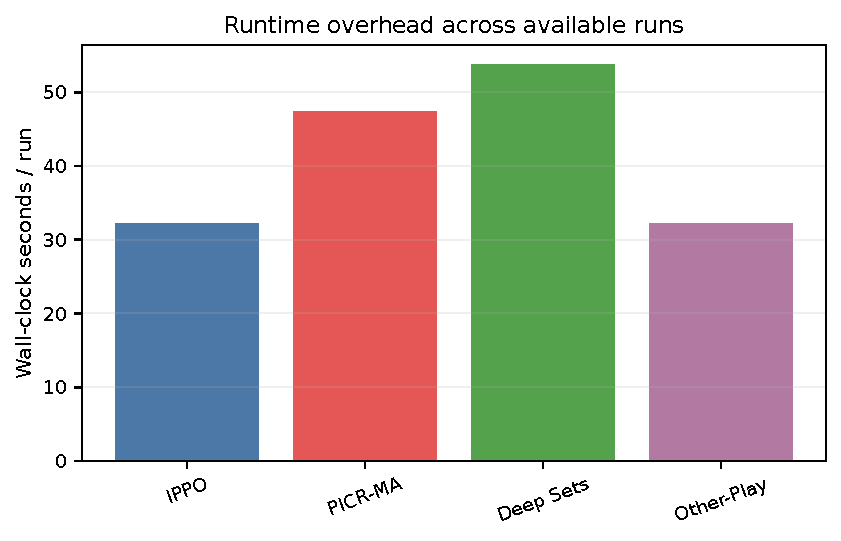
\includegraphics[width=\linewidth]{latex/figures/runtime_overhead.pdf}
\caption{Observed wall-clock runtime across the available runs.}
\label{fig:runtime-overhead}
\end{figure}

\begin{figure}[t]
\centering
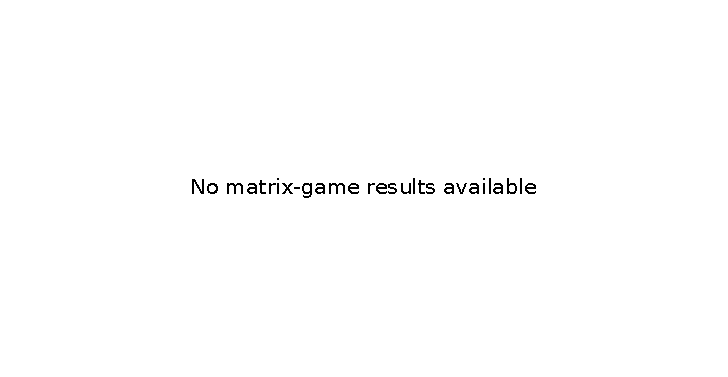
\includegraphics[width=\linewidth]{latex/figures/optional_matrix_games_summary.pdf}
\caption{Matrix-game summary under the current small-compute regime.}
\label{fig:matrix-summary}
\end{figure}
The 20k lambda sweep shows a clear tradeoff. The mild setting $\lambda{=}0.02$ gives the best PICR-MA held-out cross-play among the sweep values, matching or slightly improving IPPO on the pilot environments, while larger $\lambda$ values reduce JS more strongly but consistently hurt \texttt{simple\_spread\_v3}. Teammate dropout with probability $0.1$ is uniformly harmful in the 20k pilot, reducing cross-play on both MPE tasks and therefore does not strengthen the method. Runtime overhead is non-trivial but moderate: at 50k steps, \method\ is roughly 1.6$\times$ IPPO on \texttt{simple\_spread\_v3} and 1.3$\times$ IPPO on \texttt{simple\_adversary\_v3}, while remaining lighter than Deep Sets on \texttt{simple\_spread\_v3}. Matrix games remain useful sanity checks but do not drive the headline claim because the MPE outcomes are mixed.

\section{Discussion and Limitations (to accompany Results)}
\label{sec:discussion}
The present evidence does not support \method\ as a new default for order-sensitive MARL. The method appears most credible as a small architectural-free regularizer that can help in some cooperative settings with asymmetric partner uncertainty, but its gains are neither uniform nor robust enough to dominate stronger baselines. In particular, the method loses to IPPO, Deep Sets, and Other-Play on \texttt{simple\_spread\_v3}, and the relationship between lower permutation sensitivity and better cross-play is weaker than the motivating story would suggest.

There are several important limitations. First, the implementation uses a lightweight NumPy learner rather than a standard PyTorch PPO stack; while this keeps the artifact lean-safe and fully reproducible on a laptop, it weakens external credibility relative to a more conventional training stack. Second, the 50k-step MPE runs are materially stronger than the original 1k-step scaffold, but the learning curves on \texttt{simple\_spread\_v3} are still improving late in training, so the final scale remains modest by conference standards. Third, the method is sensitive to the regularization weight: larger $\lambda$ values improve invariance diagnostics but can reduce cross-play substantially, and teammate dropout does not rescue this behavior. These limitations are central to the internal review outcome and should temper any claim of broad effectiveness.

\section{Broader Impact}
By reducing brittle dependence on arbitrary ordering artifacts, \method can make cooperative MARL deployments more robust and reproducible with minimal engineering overhead. However, improved zero-shot coordination may also accelerate deployment of multi-agent systems in settings where safety assurances and oversight are immature; careful risk assessment is warranted.

\section{Reproducibility Statement}
We will release all code, configuration files, and scripts to reproduce figures and tables. Experiments are intentionally small-scale, use publicly available environments, and rely on fixed random seeds with logged hyperparameters. No proprietary datasets are used.

\section*{Acknowledgements}
We thank the open-source maintainers of PettingZoo and users who provided feedback on early drafts.

% ------------------------
% References
% ------------------------
\bibliographystyle{icml2025}
\begin{thebibliography}{}
\bibitem[Foerster et~al.(2016)Foerster, Assael, de~Freitas, and Whiteson]{foerster2016dqncomm}
Foerster, J. N., Assael, Y. M., de Freitas, N., and Whiteson, S.
\newblock Learning to communicate with deep multi-agent reinforcement learning.
\newblock In \emph{NeurIPS}, 2016.

\bibitem[Hu et~al.(2020)Hu, Lerer, Peysakhovich, and Foerster]{hu2020otherplay}
Hu, H., Lerer, A., Peysakhovich, A., and Foerster, J.~N.
\newblock ``Other-Play'' for zero-shot coordination.
\newblock In \emph{ICML (PMLR 119)}, 2020.

\bibitem[Liu et~al.(2020)Liu, Yeh, and Schwing]{liu2020pic}
Liu, I.-J., Yeh, R.~A., and Schwing, A.~G.
\newblock {PIC}: Permutation invariant critic for multi-agent deep reinforcement learning.
\newblock In \emph{CoRL (PMLR 100)}, 2020.

\bibitem[Lowe et~al.(2017)Lowe, Wu, Tamar, Harb, Abbeel, and Mordatch]{lowe2017maddpg}
Lowe, R., Wu, Y.~I., Tamar, A., Harb, J., Abbeel, P., and Mordatch, I.
\newblock Multi-agent actor-critic for mixed cooperative-competitive environments.
\newblock In \emph{NeurIPS}, 2017.

\bibitem[Rashid et~al.(2018)Rashid, Samvelyan, {De Witt}, Farquhar, Foerster, and Whiteson]{rashid2018qmix}
Rashid, T., Samvelyan, M., {De Witt}, C.~S., Farquhar, G., Foerster, J., and Whiteson, S.
\newblock {QMIX}: Monotonic value function factorisation for deep multi-agent reinforcement learning.
\newblock In \emph{ICML (PMLR 80)}, 2018.

\bibitem[Schulman et~al.(2017)Schulman, Wolski, Dhariwal, Radford, and Klimov]{schulman2017ppo}
Schulman, J., Wolski, F., Dhariwal, P., Radford, A., and Klimov, O.
\newblock Proximal policy optimization algorithms.
\newblock \emph{arXiv:1707.06347}, 2017.

\bibitem[Sohn et~al.(2020)Sohn, Berthelot, Carlini, Zhang, Zhang, Raffel, Cubuk, Kurakin, and Li]{sohn2020fixmatch}
Sohn, K., Berthelot, D., Carlini, N., Zhang, Z., Zhang, H., Raffel, C., Cubuk, E.~D., Kurakin, A., and Li, C.-L.
\newblock FixMatch: Simplifying semi-supervised learning with consistency and confidence.
\newblock In \emph{NeurIPS}, 2020.

\bibitem[Sukhbaatar et~al.(2016)Sukhbaatar, Szlam, and Fergus]{sukhbaatar2016commnet}
Sukhbaatar, S., Szlam, A., and Fergus, R.
\newblock Learning multiagent communication with backpropagation.
\newblock In \emph{NeurIPS}, 2016.

\bibitem[Sunehag et~al.(2018)Sunehag, Lever, Gruslys, Czarnecki, Zambaldi, Jaderberg, Lanctot, Sonnerat, Leibo, Tuyls, and Graepel]{sunehag2018vdn}
Sunehag, P., Lever, G., Gruslys, A., Czarnecki, W.~M., Zambaldi, V., Jaderberg, M., Lanctot, M., Sonnerat, N., Leibo, J.~Z., Tuyls, K., and Graepel, T.
\newblock Value-decomposition networks for cooperative multi-agent learning.
\newblock In \emph{AAMAS}, 2018.

\bibitem[Terry et~al.(2021)Terry, Black, Grammel, Jayakumar, Hari, Sullivan, Santos, Perez, Horsch, Dieffendahl, Williams, Lokesh, and Ravi]{terry2021pettingzoo}
Terry, J.~K., Black, B., Grammel, N., Jayakumar, M., Hari, A., Sullivan, R., Santos, L., Perez, R., Horsch, C., Dieffendahl, C., Williams, N.~L., Lokesh, Y., and Ravi, P.
\newblock PettingZoo: Gym for multi-agent reinforcement learning.
\newblock In \emph{NeurIPS Datasets and Benchmarks}, 2021.

\bibitem[Terry et~al.(2020)Terry, Grammel, Son, Black, and Agrawal]{terry2020ps}
Terry, J.~K., Grammel, N., Son, S., Black, B., and Agrawal, A.
\newblock Revisiting parameter sharing in multi-agent deep reinforcement learning.
\newblock \emph{arXiv:2005.13625}, 2020.

\bibitem[Tarvainen and Valpola(2017)]{tarvainen2017meanteacher}
Tarvainen, A. and Valpola, H.
\newblock Mean teachers are better role models: Weight-averaged consistency targets improve semi-supervised deep learning results.
\newblock In \emph{NeurIPS}, 2017.

\bibitem[Zaheer et~al.(2017)Zaheer, Kottur, Ravanbakhsh, Poczos, Salakhutdinov, and Smola]{zaheer2017deepsets}
Zaheer, M., Kottur, S., Ravanbakhsh, S., Poczos, B., Salakhutdinov, R., and Smola, A.~J.
\newblock Deep Sets.
\newblock In \emph{NeurIPS}, 2017.
\end{thebibliography}

% ------------------------
% Appendix (optional)
% ------------------------
\appendix
\section{Practical Slicing for MPE Observations}
In MPE, other-agent features appear in a fixed order. A thin wrapper precomputes per-block indices once (via environment metadata) and applies random permutations per minibatch using tensor \texttt{view}/\texttt{gather}. We will release a helper that auto-detects block boundaries from PettingZoo’s observation function \citep{terry2021pettingzoo}.

\section{Pseudocode Snippet (Current NumPy On-Policy Variant)}
\begin{algorithm}[H]
\caption{Core training step with permutation KL}
\begin{algorithmic}[1]
\STATE Given minibatch tensors: observations $O \in \R^{B\times d}$, actions $A$, advantages $\hat{A}$.
\STATE Split $O$ into $S$ and teammate blocks $U$ using precomputed indices.
\STATE Sample two permutations for each batch element and build $U^{(1)}, U^{(2)}$.
\STATE $P_1 = \pi_\theta(\mathrm{concat}(S, U^{(1)}))$, $P_2 = \pi_\theta(\mathrm{concat}(S, U^{(2)}))$.
\STATE $\mathcal{L}_{\text{\method}} = \lambda\, \mathrm{mean} \big( \KL(P_1\Vert P_2) + \KL(P_2\Vert P_1) \big)/2$.
\STATE Compute PPO loss and add $\mathcal{L}_{\text{\method}}$. Optimize.
\end{algorithmic}
\end{algorithm}

\end{document}
